\subsection{Method Overview}

This section details our method for achieving the goals laid out in Section \ref{objectives}. The objective is to identify map points which, while previously viewed, are no longer visible due to environmental changes. To address this, we assign an incrementally updated probability of existence value to each map point. Observations of a map point increase our overall confidence in its existence. Conversely, failure to observe a map point from a viewpoint where it \textit{should} have been visible lowers our confidence in its existence. Determining whether a map point should be observable from a given viewpoint is not trivial, motivating the need for a viewpoint-aware observability model. The purpose of the model is to integrate historical observability data to estimate observability across all possible viewpoints.

\subsubsection{The Observability of Map Points}

For the purposes of KV-SLAM, map features can be conceptualized as static, infinitesimally small points in 3D space. Because they have no width or height, a map feature can never be partially obscured, and are immune to perspective. This means that the visibility of a map feature can be represented by the function
$$
    v:(\theta,\phi,d):[0,2\pi)\times\left[-\frac{\pi}{2},\frac{\pi}{2}\right]\times[0,\infty)\to{0,1}
$$
where $\theta\in[0,2\pi)$ represents the azimuth, $\phi\in\left[-\frac{\pi}{2},\frac{\pi}{2}\right]$ represents the elevation, and $d\in[0,\infty)$ represents the distance between the map feature and the observer. This visibility function returns 1 if the point is observable from the input viewpoint, and 0 if it is not. For illustrative purposes, The left plot of Figure \ref{fig:2d_observability} represents the output of a simplified 2D version of the observability function and the effects of obstructions on the observability. However, to generate such a plot from sensor data would require infinite observations. Instead, the system must operate on a finite set of observations like the plot shown on the right. As the overall confidence in the point's existence will be updated using a Bayesian update step, the model should produce an estimate $P()$

\begin{figure}[!ht]
    \centering
    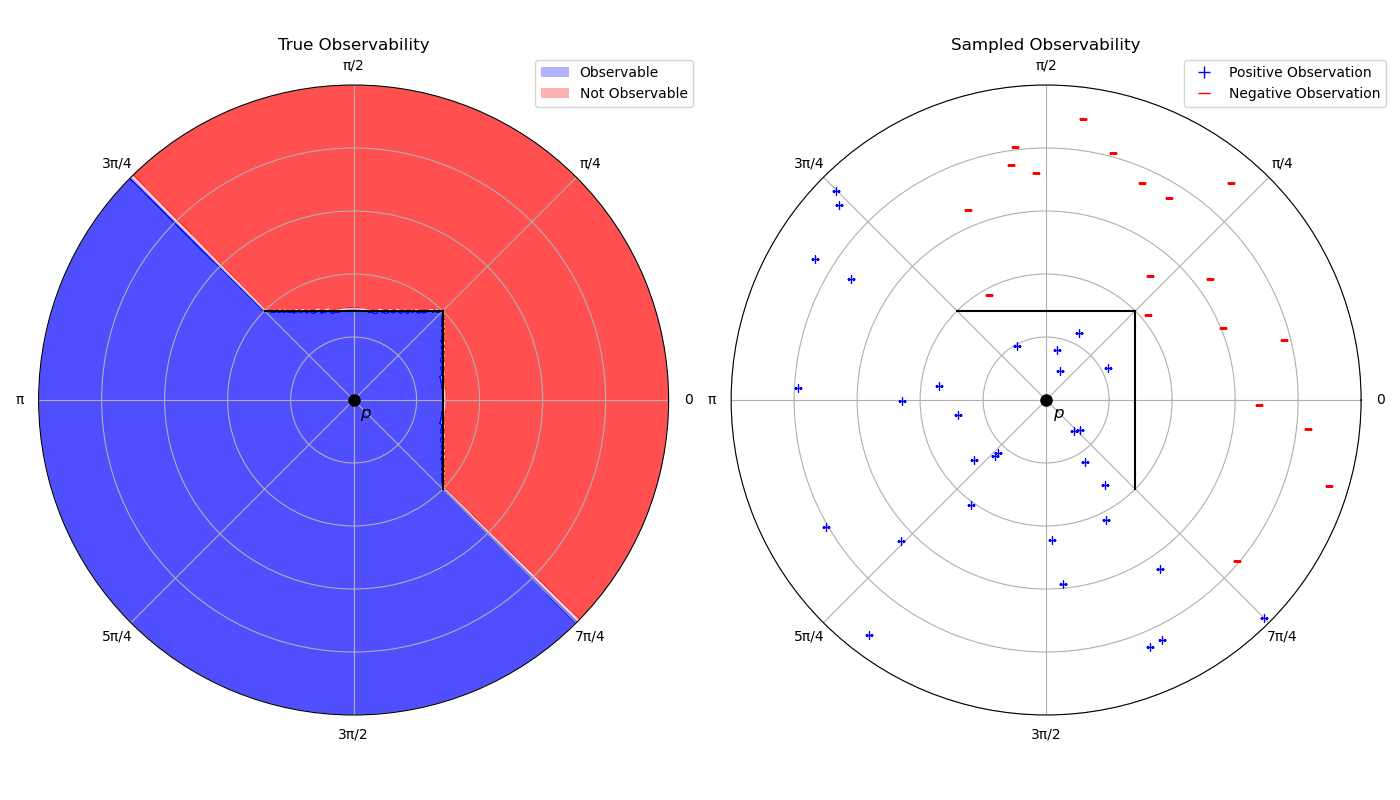
\includegraphics[width=0.9\textwidth]{resources/2d_observability.png}
    \caption[2D Observability]{(Left) A 2D representation of a map points observability when near two orthogonal obstructions. }
    \label{fig:2d_observability}
\end{figure}

\subsubsection{Modeling Historical Map Point Observability}

The goal of the model is to estimate the observability of a point using a finite set of $n$ observations O, and a current viewpoint. Observations take the form $o_n={theta_n,\phi_n,d_n,seen_n}$, so the model can be written
$$
    m(\boldsymbol{O},\theta,\phi,d)\to[0,1]
$$

The goal of the model is to minimize the total error between the model's estimate of the observability across the domain and the actual observability across the domain
$$
    minimize(sum(abs(m(\boldsymbol{O},\theta,\phi,d)-v(\theta,\phi,d)))) across the full domain
$$

Three implementations of the model $m$ will be implemented, and will have their parameters optimized in simulation. Each will be tested on the datasets produced for this research. With perfect sampling,

\subsubsection{Modeling Historical Map Point Observability}
\label{sec:observability_models}
% define what we mean by viewpoint aware observability; a mapping between observation unit direction vector and seen/not seen binary observations

We define viewpoint aware observability as a function
\begin{align*}
    \boldsymbol{f:}\mathbb{S}^2\times\mathbb{R}^+\rightarrow\{0,1\}
\end{align*}
where $\mathbf{v}\in\mathbb{S}^2$ is a unit direction vector pointing from the map point to the observer, and $d\in\mathbb{R}^+$ is the Euclidean distance between the point and observer. The function $\boldsymbol{f}(\mathbf{v}, d)\rightarrow\{0,1\}$ returns 1 if the map point is considered visible from that viewpoint, and 0 otherwise.

% Justify why distance needs to be accounted for, use a diagram to show that by including distance, we can account for occlusions in the model

The inclusion of distance in the model is necessary to handle occlusions in the environment. Figure \ref{fig:enhanced_general_slam_pipeline} shows a situation. By integrating distance data into the model, we can accurately determine whether an observation warrants modifying the point's probability of existence, or if it should be considered occluded.

% Say what we are trying to build; a model which can produce a probability that a point will be seen given an observation direction and a distance

The model operates in two stages: the observation stage, and the query stage. Observations modify the model's internal representation of a map point's observability, while queries ask \"What is the probability that I see the map point from this viewpoint?\". The observation function operates on observation data in the form $\boldsymbol{o} = \{\boldsymbol{v}\in\mathbb{S}^2\times d\in\mathbb{R}^+\times o\in\{0, 1\}\}$, where $\boldsymbol{v}$ represents the unit vector pointing from the map point to the observer, $d$ represents the distance between the map point and the observer, and $o$ represents whether the map point was seen or not. The query function operates on a similar set of parameters, excluding the observation success, represented as $\boldsymbol{q} = \{\boldsymbol{v}\in\mathbb{S}^2\times d\in\mathbb{R}^+\}$. The goal of the model is to provide answers to queries which are as accurate as possible based on the observations received up until that point. With perfect knowledge of the map point's observability across the domain of viewpoints, every query response would be a 0 or a 1, however, this would require infinite observations to produce. Instead, we implement the model probabilistically, allowing a finite number of observations to estimate the point's observability across the domain, and returning a probability of observation in the range [0, 1]. Figure \ref{fig:2d_observability} provides a simplified 2D representation of a map point $\boldsymbol{p}$'s ideal observability.



\subsubsection{Observability Shell Representations}

We model the viewpoint-aware observability of each map point using a geometric shell representation. This shell structure encodes the directional observation history of the point and is incrementally updated as new observations are processed. The shell can be implemented using various geometric constructs, and in both continuous and discrete modalities. This work proposes two observability shell representations: a discrete version implemented on an icosahedral shell, and a continuous version implemented on a spherical shell. For both structures, observation and query functions are provided.

The discrete icosahedral shell allows the full observation history to be integrated into a set of discrete bins, requiring constant additional space per map point. On the other hand, the continuous model stores data for each observation, meaning the space requirements increase with time. This growth can be bounded by limiting the number of stored observations, for example using a fixed size queue.

Below we introduce the mathematical formulation for both the discrete and continuous shells. For each modality, the mathematics behind the observation and query functions are defined and discussed.

\paragraph{Discrete Icosahedral Shell}

The icosahedron was selected for the discrete shell because it contains the highest face count of the convex Platonic solids. This provides 20 bins across the domain of viewpoints, each with identical coverage of the domain.

\subparagraph{Icosahedral Shell Formulation}

For the purposes of the mathematical formulation of the observation and query functions, the geometric details of the icosahedral shell are not relevant. The specifics of the geometric construction used in this work are discussed in Section \ref{sec:icos_construction}.

Let $M=\{mp_i\}_{i=0}^{n_{mp}}$ represent a map $M$ containing $n_{mp}$ map points. We define $S_i=\{F_{i,j}\}_{j=1}^{20}$ to represent the icosahedral shell $S$ attached to $mp_i$, containing 20 faces $F_{i,{1..20}}$. Finally, we define $F_{i,j}=(d_{i,j}, p_{i,j})$ where $d_{i,j}\in\mathbb{R}^+$ represents the maximum distance through which $mp_i$ has been observed through face $F_{i,j}$, and $p_{i,j}\in[0,1]$ represents the probability of observing $mp_i$ through face $F_j$.

Additionally, we require a function $\phi:\mathbb{S}^2\rightarrow\{1..20\}$ which maps unit vectors to the face through which they point. This function can be defined as follows:
$$
    \phi(\mathbf{v}\in\mathbb{S}^2) = \underset{j\in\{1..20\}}{\arg\max}(\mathbf{v} \cdot \boldsymbol{f}_{i,j})
$$
where $\boldsymbol{f}_{i,j}$ represents the unit vector pointing from $mp_i$ to the centroid of face $F_{i,j}$.

With these constructs in hand, we can define the observation and query functions for the icosahedral shell.

\subparagraph{Observation Function Formulation}

The observation function operates on observational inputs of the form $\{\boldsymbol{v}\in\mathbb{S}^2\times d\in\mathbb{R}^+\times o\in\{0, 1\}\}$. If the observation is successful ($o = 1$), $n_{seen}$ is incremented for $F_{i,j}$, and $p_{i,j}$ is recalculated using the formula
$$
    p_{i,j}=\frac{n_{seen}}{n_{seen}+n_{unseen}}
$$
On the other hand, if the observation is unsuccessful, we first determine if the point is observable from this distance and viewpoint. If it is not, no further actions are taken. This failed observation is likely due to a real, physical occlusion in the environment.

\subparagraph{Query Function Formulation}

\paragraph{The Continuous Shell Representation}


\subsubsection{Existence Probability and Update Rule}
\label{sec:existence_confidence}

\subsubsection{Application to Point Pruning and Selection}
